\documentclass[10pt,english]{article}
\usepackage{bookmark}
\usepackage{geometry}
\usepackage{anyfontsize}
\usepackage{lmodern}
\usepackage{lipsum}
\usepackage{sectsty}
\usepackage{amsmath}
\usepackage{amssymb}
\usepackage[T1]{fontenc}
\usepackage[utf8]{inputenc}
\usepackage[explicit]{titlesec}
\usepackage[sfdefault]{inter}
\usepackage{sfmath}
\usepackage{hyperref}
\usepackage{enumitem}
\usepackage{listings}
\usepackage[final]{graphicx}
\usepackage{subfig}
\usepackage{array}
\usepackage[table]{xcolor}
\usepackage{tikz}
\usepackage{graphicx}
\usepackage{csvsimple}
\graphicspath{{./images/}}
\usepackage[explicit]{titlesec}


\linespread{1.2}
\title{\huge{\textbf{Spotting}}}
\author{
    \\\\
    David Hermanto\\
    \small 3808127\\
    \\
    Rafat Mahiuddin\\
    \small 3897093\\
    \\
    Harry Porter\\
    \small 3888604\\
    \\
    Adrian Rebellato\\
    \small 3889401\\
    \\
    Myeonghoon Sun\\
    \small 3774430\\
    \\\\
}
\date{}

\begin{document}

\maketitle
\thispagestyle{empty}
\clearpage

\vspace*{\fill}
\begin{center}
\includegraphics[scale=0.1]{images/9DDC331C-9A71-4E19-AECC-54D8ED6C2240.png}
\end{center}
\vfill
\thispagestyle{empty}

\clearpage

\pagenumbering{arabic}

\section*{Solution}

In this section, we first discuss the components and architecture of our software, then our methodology with respect to meeting the project requirements.

% Where should this go? Probably interspersed throughout the report.
% Positions the work within the literature.
% Compares the project to other appropriate state-of-the art methods.

\subsection*{Structure}

% Technical description of project:
% Software, launch files, configuration, and implementation.
% Description of the implemented software.
%   Requires:
%   - Excellent and complete technical description of the ROS package components.

The following packages are entirely our creations, outside the Python and ROS dependecies used in their implementation.

\begin{itemize}[noitemsep]
    \item \texttt{spot\_compose} Entry point package used to execute Spotter's dependencies.
    \item \texttt{spot\_conductor} Conducts higher order actions in a synchronised fashion while acting as a gatekeeper to the rest of the architecture. Currently, the \texttt{Conductor} is tasked with camera calibration and orchestrating a good initialisation procudure for occupancy grid generation. It is also capable of enforcing the robot's desired behaviour throughout execution, however this functionality is not fully implemented yet.
    \item \texttt{spot\_cartographer} The \texttt{Cartographer} is responsible for managing the diverse library of maps created by our slam algorithm. As our operations must be persitent across maps, it is important to have a module that manages these changes directly. The \texttt{Cartographer} also controls the flow of point cloud data to the mapping pipeline.
    \item \texttt{spot\_geography} The geography package is a collection of pipelines responsible
    for filtering, evaluating, storing and processing point clouds. The primary purpose for the geography pipeline is to take in a point cloud stream and convert it to a usable occupancy grid for navigation. The geography pipeline depends on the \texttt{octomap} ROS package to create, store and load octrees based on their proposed \texttt{octreee} encoding algorithms. The usage of \texttt{octomap} as a dependency and possible replacements are discussed later on in this report.
    \item \texttt{spot\_move} represents a cohesive package for all of Spot's navigation. Every function acts as an interface betweena \dots The \texttt{Navigator} recevies a heavily pre processed two-dimensional occupancy grid with the objective of creating a safe path around obstacles on that grid. The primary path planner used by the \texttt{Navigator} is \texttt{D* Lite}, which allows for efficient recomputation of the path to support remapping dynamic environments.
 spot ros and the spotters program. The movement package allows for a standradised set of methods to execute robot mvoement in a controlled, and centralised manner. The movement package also allows for robot safety, since only the spot move should move the motors on spot, spot will always stop moving if that node is killed.
    \item {}\end{itemize}

Modified third party.

\begin{itemize}
    \item \texttt{spot\_ros}
    \item \texttt{spot\_slam}
    \item \texttt{spot\_description}
    \item \texttt{spot\_viz}
\end{itemize}

Entirely third party.

\begin{itemize}
    \item \texttt{spot\_wrapper}
    \item \texttt{spot\_msgs}
    \item \texttt{spot\_cam}
    \item \texttt{spot\_driver}
    \item \texttt{octomap\_server}
    \item \texttt{usb\_cam}
\end{itemize}



\clearpage

\subsection*{Architecture}

% Description of the of Robot Software Architecture.
% Excellent and complete.

% Justification of the choice of Robot Software Architecture.
%   Requires:
%   - Excellent justification of the Robot Software Architecture.
%   - Well-supported reasoning.

Here we outline the overarching structure of our system; the behaviours of each constituent part are described in the next section, often with reference to these diagrams.

\clearpage

\subsection*{Methodology}

% Describe methodology and approach towards completing the negotiated requirements of the project.
%   Requires:
%   - Excellent description of methodology.
%   - Provides a complete picture of how the project is completed.

Here we discuss the intended and implemented behaviours of all our custom packages, and how they fit into the overall pipeline to produce navigation over an occupancy grid derived from visual information.

\subsubsection*{Localisation \& Mapping}

Our localisation and mapping processes are based on the \texttt{ORB-SLAM3} algorithm [1] and package [?]. % Need to reference the repository.

\subsubsection*{Occupancy Grid Generation}

Our strategy for generating a navigable occupancy grid is a geometric one. First, a two-dimensional slice is taken from the \texttt{octree} point cloud and sent to our mapping pipeline as an \texttt{OccupancyGrid} message. All coordinates where features have been identified are obstructed in the occupancy grid; these coordinates are taken and used as the vertices in our Delaunay triangulation process that producess alpha shapes over sufficiently dense clusters of features. Alpha shapes are collections of linear curves which outline the shape of a finite set of coordinates.

Delaunay triangulation is the production of edges over a set of points such that the edges create triangles and the circumcircles of each triangle do not contain any additional points. The result is effectively a triangular mesh over the two-dimensional slice generated from the point cloud. This mesh is then polygonised -- internal edges are removed and external edges combined into a single shape -- using Python's \texttt{Shapely} library, where each polygon thus represents an intraversible region in the environment. This transforms the sparse point cloud, where walls and other obstructions are often permeable due to the low density of features, into the navigable map where obstructions are contiguous. A configurable alpha value is used to constrain the size of each shape in the triangulation, so points that are sufficiently separated are not subsumed by a single polygon in the next step. At present, this value has been configured manually, but we believe it possible to calculate the optimal alpha for a given set of points. We have not looked into this extensively, though.

Once these occlusion polygons have been generated, we translate the occluded and free space back into a two-dimensional array. Initially, this was done by taking every index and testing if the corresponding coordinate was inside any of the generated polygons using \texttt{within} or \texttt{contains} from the \texttt{Shapely} library. However, this quickly becomes untenable for larger maps because these functions are quite expensive, and confirming that a cell is not occupied requires verifying that it is not inside any polygon. To speed this process up, we have used a data structure from Python's \texttt{rtree} library that performs spatial queries very quickly. By storing all polygons inside this \texttt{rtree}, we can very quickly narrow down the number of polygons that need searching for each point by querying possible matches. We then check each possible match for containment of the point using \texttt{Shapely} as before, where the number of invocations has been substantially reduced.

Once this process is complete and all points in the occupancy grid have been marked as free or occupied, the array is reshaped into one dimension and published as a new \texttt{OccupancyGrid} message. This process allows us to map from a sparse point cloud by treating clusters of features as contiguous, and therefore non-navigable shapes. However, we believe a much faster method exists for deriving the occupancy grid from the generated polygons; we have discussed this as part of our analysis.

\subsubsection*{Navigation}

The navigation pipeline is heavily based on the \texttt{D* Lite} heuristic search algorithm.
We have chosen the \texttt{D* Lite} as our path-finding algorithm since it is considered optimal, complete, and computationally efficient as compared to other path-finding algorithms [2].
Compared to \texttt{A*}, \texttt{D* Lite} is considered more efficient in such complex environments as the interiors of the hospital where paths need to be recalculated as the robot traverses and runs into new obstacles it was not aware of prior.

We have utilised an existing algorithm [3] and modified it so that it can be integrated into the rest of our architecture. Following details how our customised path planner works.
Once the current position, the goal position, and the map are known, the path planner package creates a navigation task object to initiate the path-finding using \texttt{D* Lite}.
Since the existing algorithm uses a two-dimensional array, the published one-dimensional map data need to be reshaped, thereby making it necessary to convert published poses into corresponding rows and columns in the two-dimentional array. Via rostopics, the navigation task object stores all the data, converted or original, needed to initiate the path-finding.

Once the navigation task is initiated, the robot's initial movement according to the path generated by \texttt{D* Lite} helps dynamically update the path based on the newfound, neighbouring cells in the viewing range. The viewing range itself is dynamic to the map resolution, tuned to make sure that the robot doesn't waste resources trying to plan too far ahead, but still being able to comfortably walk around obstacles close by. The navigation pipeline then continues to publish updated paths until the current position of the robot is close to the goal position by some constant threshold, after which another navigation task will be created and wait for the necessary data to begin another episode of path-finding.

Because of the nature of the \texttt{ORB-SLAM3} algorithm, it is likely that the robot will lose its localisation from time to time. To accommodate a situation like this, we have used the rostopic to publish boolean data to recover the goal position previously set before the localisation was lost. We also make sure to bound our goal position within the map, and the ultimate goal is cached so that we can progressively get closer to it. With D* Lite, every time a new map is received, cells within the viewing range of the current position cell are factored in to generate an updated path. This process is repeated until the final goal is reached.


\subsubsection*{Planning \& Behaviour}

Our \texttt{Conductor} manages the state, and thus the appropriate behaviour, of our robot in its environment. It is effectively an automaton with the following states:

\begin{itemize}[noitemsep]
    \item \texttt{START} is the initial state upon startup. At present, given the absence of any initial navigable map, this state encodes behaviours that helps our visual mapping solution generate one, such as turning around slowly and moving to get different perspectives of the same environment. States outside this one are generally only entered after this initial map has been built. If a map is available, this state transitions to \texttt{GOAL} if a navigation goal has been received, or \texttt{IDLE} otherwise. It's worth noting that these initial behaviours would be made redundant by a more reliable and accurate visual mapping system; we have discussed these details in our analysis.
    \item \texttt{GOAL} is the state entered upon the receiving a navigation goal, and which persists until either that goal is reached, cancelled, or localisation in the current occupancy grid is lost. The behaviour in this state is navigation toward the given goal position: this is achieved by receiving a path -- either to the coordinate itself, or to the nearest known location in the event that a map of the area doesn't exist yet -- as a sequence of poses from \texttt{Navigation} and dispatching the corresponding gRPC calls to Spot via the \texttt{ros\_wrapper} package.
    \item \texttt{LOST} is the state entered when localisation is lost, and is intended to encode behaviours that will help re-establish localisation, such as looking and moving around to identify features. These behaviours were deemed surplus to requirements for submission, but the framework for their implementation remains.
    \item \texttt{IDLE}  % TODO: Finish talking about these states.
    \item \texttt{RECOVER}
\end{itemize}

The transition diagram of these states is as follows. Not all of these transitions are implemented at the moment, but these are the intended behaviours.

\begin{center} % TODO: Finish this state diagram.
    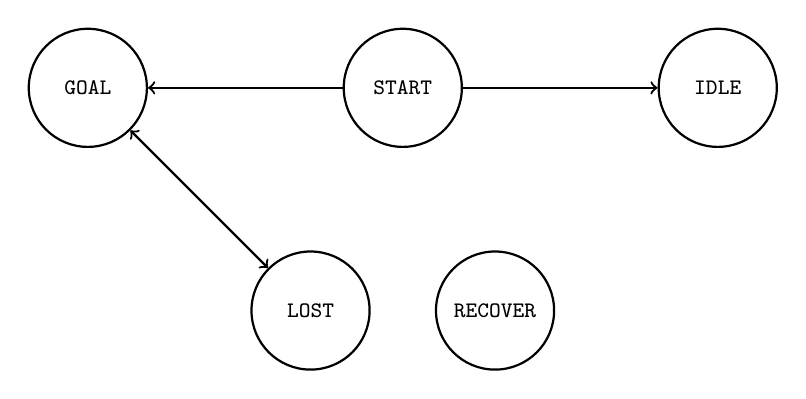
\begin{tikzpicture}[main/.style = {draw, circle}, node distance={40mm}, thick, minimum size=1.5cm]
        \node[main] (1) {\footnotesize \texttt{START}};
        \node[main, right of=1] (2) {\footnotesize \texttt{IDLE}};
        \node[main, left of=1] (3) {\footnotesize \texttt{GOAL}};
        \node[main] (4) [below right of=3] {\footnotesize \texttt{LOST}};
        \node[main] (5) [below left of=2] {\footnotesize \texttt{RECOVER}};
        \draw[->] (1) -- (2);
        \draw[->] (1) -- (3);
        \draw[<->] (3) -- (4);
    \end{tikzpicture}
\end{center}

\clearpage

\section*{Retrospective}

\subsection*{Analysis}

% Analysis of the strengths and weaknesses of the software.
%   Requires:
%   - Excellent analysis of the final deliverable.
%   - Provides a clear understanding of the strengths and weakness of the software.

\subsubsection*{Occupancy Grid Generation}

Whilst our technique for generating a navigable occupancy grid over a sparse point cloud has been serviceable for testing so far, our testing environments have been quite small and open for the most part. We are quite sure that performance would degrade significantly when navigating around a larger map, because more polgons are generated and more points need to be tested for membership of those polygons. So, our current solution does support the deliverable of producing a map of the environment that can be used for navigation, but it is unlikely to scale very well.

The key strength of our technique in this area is the coagulation of clustered points into contiguous polygons that are impermeable from a path planning perspective. This transforms the sparse point cloud generated by our VSLAM algorithm into a useful model of the environment. However, not only are the constituent computations rather expensive, but the entire map is recomputed whenever more data is incorporated from the camera. This means, as mentioned before, that performance degrades sharply for maps of larger areas. Ideally, only a surrounding region of our map would be recomputed for every new frame of information, instead of the whole map, but we have not considered this in depth at this stage.

There is also a technique we've theorised for substantially increasing the speed of occupancy grid generation once the polygons have been derived. At the moment, every position in the two-dimensional occupancy grid needs to be checked occlusion by a polygon. As a temporary solution, we have reduced the number of cells checked artificially, by checking every third location across both axes and occluding the nine surrounding cells if an obstruction is found for each check. This is very undesirable in the long term because it drastically reduces map resolution, and could lead to occlusions being undetected or overestimated. This is especially true in the case of doorways, for example, which could become completely blocked in the occupancy grid as a result of this low-resolution sampling. More detail in our occupanyc

\subsubsection*{Navigation}

There are several strengths and weaknesses of the approach with \texttt{D* Lite} implementation.

When provided with a goal that is out of bounds of the currently known area, it will successfully continue to publish a path plan towards the closest possible point towards the goal until it receives new knowledge about the map, in which case it will re-plan even further towards the goal. Another strong point is that it successfully handles all situations where the robot might be out of bounds, or no path could be planned, and alerts the user during such conditions. This leads to the navigation system being able to tolerate and handle situations where the map being published is not completely accurate.

However, there are also some weaknesses with the current approach, of which one would be sync problems with the other publishers. When the robot gets lost, the old map would be temporarily set aside until the robot successfully localizes and merges the maps back together. This is an issue, as when a path calculation happens at the same time as the map is being replaced with a completely new one, the planner might be really off, or simply not work at all due to it reading the modified data halfway through the calculation. This issue is an edge case and will not happen often. A way to fix it would be to turn off everything related to updating the map while the path calculation is being done. While this will fix the planner stopping, it might generate a wrong path if the robot is lost by a huge displacement until the next time path is calculated, and as such, is not a perfect solution.

\clearpage

\subsection*{Evaluation}

% Critical evaluation of the project in relation to the negotiated requirements.
% Quality of quantitative and/or qualitative experimental results.
%   Requires:
%   - Excellent evaluation of the capabilities of the final deliverable.
%   - Well-supported experimental evidence.

\subsubsection*{Occupancy Grid Generation}

Overall, the technique we've used for generating a navigable occupancy grid over a sparse point cloud has been sufficient for the robot to map and navigate its environment.

\subsubsection*{Navigation}

The navigation part within the project pipeline has done an adequate job of providing the robot with the path it needs to take towards the goal. Tests were run using a tool called \textit{rosbag}, which allows ROS topics to be recorded and replayed at anytime. Within these testing environments, various conditions were tested to see whether the navigation system would come up with the correct paths:

\begin{enumerate}[noitemsep]
    \item Attempting to plan a path when there is a clear path available. This results in a path being generated as expected, generating a path around obstacles within viewing range, but not looking too far ahead. % NEED PICTURES REFERENCED
    \item Attempting to plan a path out of bounds. This results in a path being generated to the edge of the known area leading towards the goal, which is the expected behaviour.
    \item Attempting to plan into an obstacle outside of viewing range. This results in a path being generated as if there were no obstacles. When the goal comes into viewing range, the navigation system decides that no path is possible and stops planning, which is the ideal behaviour.
    \item Attempting to plan a path towards a goal, then getting lost. After receiving the new dummy map, the system sets the goal to a distance relative to where it was before getting lost, which is the intended behaviour of the goal persistence behaviour.
\end{enumerate}

Later on, tests would be run directly on the robot itself while following the path with similar outcomes. An issue that pops up is that the robot would get lost often and the navigation system would become imprecise. % SHOW PICTURES SOMEWHERE?

\clearpage

\vspace*{\fill}
\begin{center}
\includegraphics[scale=0.1]{images/429F1310-292D-47FB-AB48-3564D69C3279.png}
\end{center}
\vfill
\thispagestyle{empty}
\clearpage

\section*{Contributions}  % Add your contributions here.
\clearpage

\section*{References}

\begin{enumerate}[leftmargin=*,label={\texttt{[\arabic*]}},noitemsep]
    \item C. Campos, R. Elvira, J. J. G. Rodríguez, J. M. M. Montiel and J. D. Tardós, ``ORB-SLAM3: An Accurate Open-Source Library for Visual, Visual-Inertial, and Multimap SLAM,'' in IEEE Transactions on Robotics, vol. 37, no. 6, pp. 1874-1890, Dec. 2021, doi:\\10.1109/TRO.2021.3075644.
    \item P. E. Teleweck and B. Chandrasekaran, ``Path planning algorithms and their use in robotic navigation systems,'' Journal of Physics: Conference Series, vol. 1207, p. 012018, 2019, doi:10.1088/1742-6596/1207/1/012018
    \item Sollimann, ``Sollimann/Dstar-Lite-pathplanner: Implementation of the D* lite algorithm in python for `Improved fast replanning for robot navigation in unknown terrain,''' GitHub, https://github.com/Sollimann/Dstar-lite-pathplanner (accessed Jun. 16, 2023).
\end{enumerate}

\end{document}
